\begin{solution}{Question 4}\label{ques:4}
    \begin{question}
    Let Commit be a single-bit commitment scheme. Show that if Commit satisfies the collapse-binding property, then it also satisfies prof-binding.
    \end{question}
    \tcblower{}
    \begin{proof}
    To prove that collapse binding implies prof binding, we will show a reduction where if the adversary breaks prof binding with some non negligible probability $\epsilon$, the reduction breaks collapse-binding with some non negligibile probability $\mathcal{O}(\epsilon)$. Let the games for collapse-binding and sum-binding be defined as follows:\\
    \begin{figure}[H]
      \begin{subfigure}[b]{0.5\textwidth}
        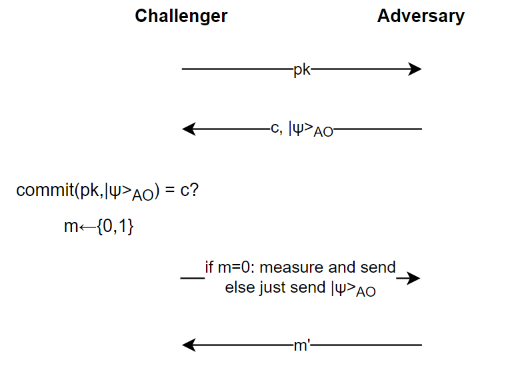
\includegraphics[width=\textwidth]{images/collapse.png}
        \caption{Collapse-binding}
        \label{fig:cb}
      \end{subfigure}
      \hfill
      \begin{subfigure}[b]{0.48\textwidth}
        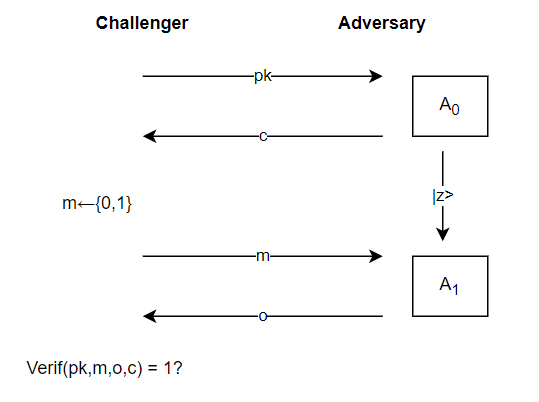
\includegraphics[width=\textwidth]{images/prof.png}
        \caption{Prof binding}
        \label{fig:prof}
      \end{subfigure}
      \caption{Games for the two commitment schemes}
    \end{figure}

    The collapse binding game is exactly as defined in the class. For prof binding, the game is same as in the classical setting but the adversary can do quantum analysis on the same. The circuits $A_0$ and $A_1$ are defined as follows with z being a quantum state obtained by $A_0$ after calculating $c$ and remaining terms having the same meaning.
    \begin{center}
        \begin{quantikz}[thin lines]
            \lstick{$pk$} & \gate[wires=2]{A_0} & \qw & \rstick{$c$}\\
            & &  \qw & \rstick{$\ket{z}$}
        \end{quantikz}
    \end{center}

    \begin{center}
            \begin{quantikz}[thin lines]
                \lstick{$\ket{b}$} & \gate[wires=3]{A_1} & \qw & \rstick{$\ket{b}$}\\
                \lstick{$\ket{z}$} & & \qw & \rstick{$\ket{z_b}$}\\
                \lstick{$\ket{\mathbf{0}}$} & & \qw & \rstick{$\ket{o_b}$}
            \end{quantikz}
        \end{center}

    \newpage
    The reduction is now defined as follows:
    \begin{figure}[H]
        \centering
        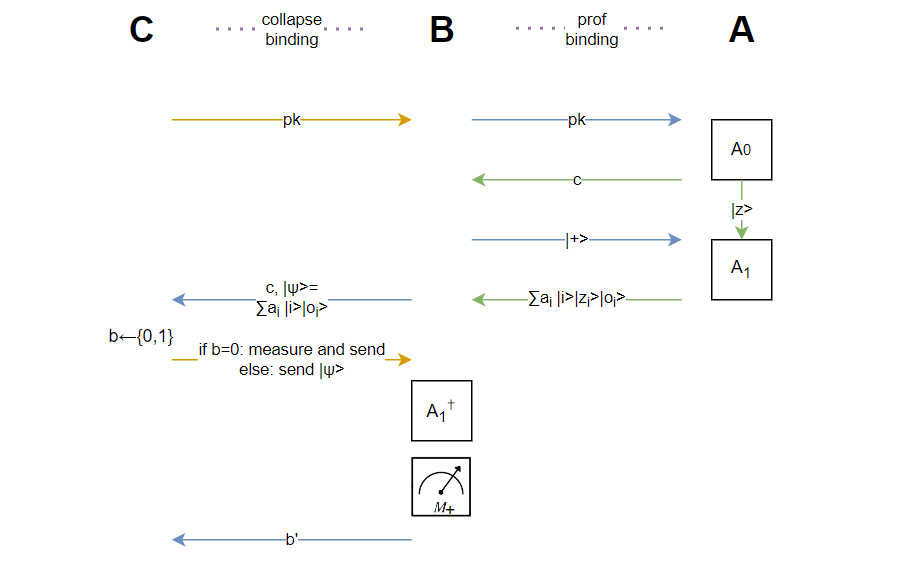
\includegraphics[width = 0.8\textwidth]{images/reduction.png}
        \caption{Reduction}
        \label{fig:my_label}
    \end{figure}

    The Reduction \textbf{B} has full access to the adversary \textbf{A} which breaks prof binding with non negligible probability $\epsilon$. Reduction forwards the public key sent by the challenger (\textbf{C}) and then interacts with \textbf{A} to obtain a superposition $\sum_i \alpha_i \ket{i}\ket{z_i}\ket{o_i}$ where $i$ can take values 0, 1. From this, \textbf{B} extracts the registers $\ket{i}$ and $\ket{O_i}$ to create $\ket{\psi}$ which is a super position of 0, 1 with their openings for the same commitment $c$. B forwards $c, \ket{\psi}$ to the challenger. Challenger checks the validity of the commitment and the openings. It then chooses a bit $b \leftarrow \{0,1\}$ and if $b=0$, it measures $\ket{\psi}$ and sends it to \textbf{B}. Else it sends $\ket{\psi}$ without measuring. \textbf{B} now analyses and sends $b'$ to \textbf{C} and succeeds with high probability.\\

    B succeeds at identifying if $\ket{\psi}$ has been measure before as it applies $A_1^\dag$ (since $A_1$ is a unitary, $A_1^\dag$ exists) to $\ket{\psi}$. If $\ket{\psi}$ was not measure before, we get exactly the $\ket{+}$ state. On measuring it along the Hadamard basis, this is confirmed and \textbf{B} outputs $b'=1$ which is true and hence succeeds with probability 1. On the other hand, if $\ket{\psi}$ was measure by \textbf{C}, we get either $\ket{0}\ket{z_0}\ket{o_0}$ state or $\ket{1}\ket{z_1}\ket{o_1}$ state, and on measuring using $\calM_+$, we so not get the $\ket{+}$ state with probability $1/2$. Therefore, in the case verification passes, \textbf{B} can distinguish measurement of $\ket{\psi}$ and hence break collapse-binding with probability $1/2 \times 1 + 1/2 \times 1/2 = 1/4$.

    Probability of verification being successful directly depends on the advantage of the adversary \textbf{A} in the prof binding game. Following a similar notion as in Blum's protocol, assuming the verification passing is $\epsilon-good$, 
    \\$\prob{\text{\textbf{B} identifies $b$ correctly }| \text{ verification is }\epsilon-good}  = 3/4$

    Therefore, if a Commit scheme satisfies the collapse-binding property, then it also satisfies prof-binding.








    
    % \begin{definition}Collapse-binding: (equivalent to the definition provided in class) \\
    % For algorithms $(A, B)$, consider the following games:
    % \begin{equation}
    %     \begin{split}
    %     \text{Game}_1 &: k \leftarrow \bfP, (S, M, U, c) \leftarrow A(k), m \leftarrow \calM(M), b \leftarrow B(S, M, U)\\
    %     \text{Game}_2 : k \leftarrow \bfP, (S, M, U, c) \leftarrow A(k), b \leftarrow B(S, M, U)
    %     \end{split}
    % \end{equation}

    % Here $S, M, U$ are quantum registers and $c,m,u$ are commitment, message and the opening respectively. $verify(k, c, m, u)$ checks if u is a valid opening for commitment c of m.  $\calM(M)$ is measurement of $M$ in the computational basis.\\

    % Now, an adversary (A, B) is collapse binding-valid for verify $iff$ for all k, $\prob{verify(k, c, m, u) = 1} =1$ when we run $(S, M, U, c) \leftarrow A(k)$ and measure $M$ in the computational basis as $m$, and $U$ in the computational basis as $u$.\\
    
    % A commitment scheme is collapse-binding iff for any qpt adversary $(A, B)$ that is collapse binding-valid for verify, $\prob{b = 1 : Game_1} - \prob{b = 1 : Game_2}$ is negligible.
    % \end{definition}
    % \begin{definition}Prof-binding: For any adversary $(C_0, C_1)$ and $m\in \{0,1\}$, 
    % \begin{equation}
    %     p_m(C_0, C_1) := \prob{\texttt{verify}(k, c, m, u) = 1 : k \leftarrow \bfP,(S, c) \leftarrow C_0(k), u \leftarrow C_1(S, m)}
    % \end{equation}
    % Where $S$ is a quantum register, and c is a classical value. $C_0$ generates the commitment and $C_1$ gets an opening u for m. The advantage of adversary is defined as: $p_0+p_1-1$
    % \end{definition}
    

    % Since the adversary is a quantum algorithm, a rewinding proof does not work, hence we will run the queries in superposition. 
    
    \end{proof}
\end{solution}
 